\section{System Model}
\label{sec:system}

We consider a LEO satellite-enabled grant-free random access system
as shown in Fig.~\ref{fig:system-multiframe}, where AFDM is adopted
to mitigate the effects of doubly dispersive terrestrial-satellite
links (TSLs) \cite{shen2025,huang2026}.
The system comprises $K$ single-antenna terrestrial devices that
communicate with a LEO satellite equipped with a uniform planar array
(UPA) consisting of $M=M_yM_z$ antennas.
During each transmission block, active devices share the same resources
for pilot transmission to the satellite.
These terrestrial devices operate without
GNSS capabilities and do not pre-compensate for delay and Doppler shifts
\cite{shen2025}.

\begin{figure}[!t]
\centering
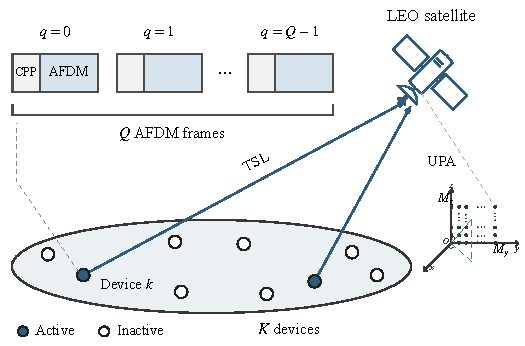
\includegraphics[width=\linewidth]{system_multiframe.pdf}
\caption{LEO satellite grant-free access with multi-frame AFDM pilot
transmission. The insets show the frame structure of active device $k$
and the satellite UPA. Device activity is fixed over the $Q$ frames.
Satellite, footprint, and array artwork
is adapted from \cite[Fig.~1]{shen2025}.}
\label{fig:system-multiframe}
\end{figure}

\subsection{Terrestrial-Satellite Link Model}

The TSLs experience fast variations due to the high mobility of the
LEO satellite. Hence, this time variation and multipath propagation
require a doubly dispersive channel model \cite{shen2025}.
We assume that the terrestrial devices are stationary and
all paths from the $k$th device have a common Doppler shift $\nu_k$
\cite{huang2026}.
Within a transmission block, the path gains, delays, Doppler shifts,
and angles of arrival remain approximately constant.
We set $t_{\rm c}=0$ at the beginning of the transmission block.
After delay compensation for $\tau_{\rm c}$ at the satellite receiver, the
channel impulse response from the $k$th device to the satellite at
time instant $t_{\rm c}$ can be represented as

\begin{equation}
 \mathbf h_k(t_{\rm c},\tau)
 =\mathbf a_k\sum_{\ell=1}^{L_k}g_{k\ell}
 e^{\mathrm j2\pi\nu_k t_{\rm c}}\delta(\tau-\tau_{k\ell}),
 \label{eq:physical-channel}
\end{equation}
where $k=1,\ldots,K$, $L_k$ is the number of physical paths,
$g_{k\ell}$ is the path gain of the $\ell$th path,
$\delta(\cdot)$ is the Dirac delta function, and $\mathrm j^2=-1$.
Here $\tau_{k\ell}=\widetilde\tau_{k\ell}-\tau_{\rm c}$ represents the
differential delay for the $\ell$th path from the $k$th device to the
satellite, where $\widetilde\tau_{k\ell}$ and $\tau_{\rm c}$ denote the
propagation delay and common delay, respectively.
The common delay corresponds to the
propagation time between the satellite and the closest point on Earth
within the beam coverage \cite{shen2025}.

The array response vector $\mathbf a_k$ at the satellite side can
be written as \cite{shen2025,li2023}
\begin{equation}
 [\mathbf a_k]_{n_z+M_zn_y}
 =e^{\mathrm j2\pi(d_yn_y\mu_{y,k}+d_zn_z\mu_{z,k})/\lambda},
 \label{eq:upa}
\end{equation}
where $n_z=0,\ldots,M_z-1$, $n_y=0,\ldots,M_y-1$,
$\lambda$ is the wavelength, and $d_v$ is the spacing between
adjacent antennas along the $v$-axis with $v\in\{y,z\}$.
Here $\mu_{z,k}$ and $\mu_{y,k}$ are the directional cosines along
the z-axis and y-axis, respectively.

\subsection{Transmission Scheme}
\label{sec:transmission-scheme}

In the proposed scheme, each active device transmits pilot symbols over
$Q$ consecutive AFDM frames within one transmission block, sharing
$N$ chirp subcarriers with the other active devices
\cite{cai2026,huang2026}.
Each frame is modulated and demodulated independently, while the
received frames are jointly processed for JADCE.
Let $\mathbf p_{qk}\in\mathbb C^N$ denote the known pilot vector of
device $k$ in frame $q$, where $q=0,\ldots,Q-1$.
The pilot vectors are collected in
$\mathbf P_k=[\mathbf p_{0k},\ldots,\mathbf p_{Q-1,k}]^{\mathsf T}$
and $\mathbf P=[\mathbf P_1,\ldots,\mathbf P_K]\in\mathbb C^{Q\times KN}$,
where $(\cdot)^{\mathsf T}$ denotes transpose.
The pilots satisfy
$\mathbf P\mathbf P^{\mathsf H}=KE_p\I_Q$, where
$\|\mathbf p_{qk}\|^2=E_p$ for all $k$ and $q$
\cite{cai2026}.
The construction of $\mathbf P$ is given in
Section~\ref{sec:simulation-settings}.

Applying the inverse discrete affine Fourier transform (IDAFT) to
$\mathbf p_{qk}$ gives the time-domain transmitted signal \cite{ding2026}

\begin{equation}
 s_{qk}[t]=\frac{1}{\sqrt N}\sum_{n=0}^{N-1}
 [\mathbf p_{qk}]_ne^{\mathrm j2\pi(c_1t^2+c_2n^2+nt/N)},
 \label{eq:afdm-time-signal}
\end{equation}
where $t=0,\ldots,N-1$, and $c_1$ and $c_2$ are AFDM modulation
parameters.
The signal in \eqref{eq:afdm-time-signal} can be represented in matrix
form as \cite{ding2026}
\[
 \mathbf s_{qk}=\mathbf F_{\rm A}^{\mathsf H}\mathbf p_{qk},
\]
where
\begin{equation}
 \begin{gathered}
 \mathbf F_{\rm A}
 =\left[\frac{1}{\sqrt N}e^{-\mathrm j2\pi(c_2r^2+rt/N+c_1t^2)}
 \right]_{r,t=0}^{N-1}
 \end{gathered}
 \label{eq:daft}
\end{equation}
denotes the discrete affine Fourier transform (DAFT) matrix.
Here $T_s=1/(N\Delta f)$ gives the sampling interval, with
$\Delta f$ denoting the subcarrier spacing.

Assume that the chirp-periodic prefix (CPP) duration is greater than
or equal to the maximum differential delay, i.e.,
$N_{\rm CPP}T_s\geq\max_{k,\ell}\tau_{k\ell}$.
Each AFDM frame spans a duration of $T_{\rm frame}=(N+N_{\rm CPP})T_s$.

For fractional delays, we use the continuous-time AFDM waveform in
\cite[Sec.~3.1.1]{bemani2023thesis} with a chirp-periodic extension over
the prefix \cite{bemani2022}.
The basis for chirp subcarrier $n$ at time $\xi T_s$ is
\begin{equation}
 \varphi_n(\xi)=\frac{1}{\sqrt N}
 e^{\mathrm j2\pi[c_2n^2+c_1\xi^2+nw_\xi/N-\zeta_n(w_\xi)w_\xi]},
 \label{eq:continuous-waveform}
\end{equation}
where $w_\xi=\langle\xi\rangle_N$,
$\langle x\rangle_N=x-N\lfloor x/N\rfloor$,
$\zeta_n(w)=\lfloor2c_1w+n/N\rfloor$, and $2Nc_1\in\mathbb N_+$.

After CPP removal and DAFT demodulation, the reference-frame channel
from device $k$ to antenna $m$ can be expressed as
\begin{equation}
 \mathbf H_{k,m}
 =[\mathbf a_k]_m\sum_{\ell=1}^{L_k}g_{k\ell}
 \mathbf G(\tau_{k\ell}/T_s,\nu_k;N_{\rm CPP}),
 \label{eq:channel}
\end{equation}
whose rows and columns correspond to received and transmitted
symbols, respectively, with $m=0,\ldots,M-1$.
Define
$\mathbf H_k=[\mathbf H_{k,0}^{\mathsf T},\ldots,
\mathbf H_{k,M-1}^{\mathsf T}]\in\mathbb C^{N\times MN}$.
For a path with gain $1$, delay $dT_s$, and Doppler shift $\nu$,
the channel response can be expressed as

\begin{equation}
 \mathbf G(d,\nu;g)=\mathbf F_{\rm A}\mathbf D_{\nu,g}\mathbf B_d,
 \label{eq:path-operator-system}
\end{equation}
where $\mathbf D_{\nu,g}=\diag\{e^{\mathrm j2\pi\nu T_s(g+t)}\}_{t=0}^{N-1}$
and $[\mathbf B_d]_{tn}=\varphi_n(t-d)$.
Here $t_{\rm c}=(g+t)T_s$ for $t=0,\ldots,N-1$ after removing
the CPP, and $g=N_{\rm CPP}$ for frame $0$.

In frame $q$, the useful samples start at
$g_q=N_{\rm CPP}+q(N+N_{\rm CPP})$. Thus,
\eqref{eq:path-operator-system} gives
\begin{equation}
 \mathbf H_k^{(q)}=e^{\mathrm jq\beta_k}\mathbf H_k,
 \label{eq:twc-frame-channel}
\end{equation}
where $\beta_k\equiv2\pi\nu_kT_{\rm frame}\pmod{2\pi}$
and $\beta_k\in[-\pi,\pi)$.
Since the paths of each device share a common Doppler shift, the
inter-frame variation is described by the scalar phase rotation
$e^{\mathrm jq\beta_k}$, while $\mathbf H_k$ remains approximately
constant over $Q$ consecutive frames.
The received signals can therefore be expressed using this shared
channel and the effective pilot matrix
\begin{equation}
 \mathbf A_k=\diag\{e^{\mathrm jq\beta_k}\}_{q=0}^{Q-1}\mathbf P_k,
 \label{eq:effective-pilot}
\end{equation}
where $\mathbf A=[\mathbf A_1,\ldots,\mathbf A_K]$.

In \eqref{eq:channel}, the effective channel at each antenna is
represented by an $N\times N$ matrix. The multi-frame OTFS scheme in
\cite[eq.~(9)]{shen2025} uses an $L\times N\times N$ tensor for $N$
subcarriers and $L$ OFDM symbols per frame. The dense AFDM channel representation
contains $MN^2$ channel entries per device, compared with
$MLN^2$ in that OTFS representation. With the same subcarrier spacing
and prefix length, $L$ AFDM frames span the duration of one OTFS
frame and contain the same number of useful samples.

\subsection{Problem Formulation}

We model device activities as independent and identically distributed
(i.i.d.) binary variables. For device $k$, define $\alpha_k$ as
\cite{cai2026}
\[
 \alpha_k=\begin{cases}
 1,&\text{if the $k$th device is active},\\
 0,&\text{otherwise}.
 \end{cases}
\]
Let $\rho$ represent the probability of a device being active, i.e.,
$\Pr(\alpha_k=1)=\rho$, where $\rho\ll1$.
As a result, only a small subset of the devices is active in any given
transmission block. The activity states are
assumed to remain constant within a transmission block.
Let $\mathbf X_k=\alpha_k\mathbf H_k$.

The received symbols in frame $q$ after CPP removal and DAFT demodulation
are collected in $\mathbf Y_q\in\mathbb C^{M\times N}$, with noise matrix
$\mathbf W_q$ containing independent $\CN(0,\sigma^2)$ entries.
Across the transmission block, the received frames form
$\mathbf Y=[\vect(\mathbf Y_0^{\mathsf T}),\ldots,
\vect(\mathbf Y_{Q-1}^{\mathsf T})]^{\mathsf T}$, with $\mathbf W$ arranged in the same way.
With $\mathbf X=[\mathbf X_1^{\mathsf T},\ldots,
\mathbf X_K^{\mathsf T}]^{\mathsf T}$, the received signal is
\begin{equation}
 \mathbf Y=\sum_{k=1}^K\mathbf A_k\mathbf X_k+\mathbf W
 =\mathbf A\mathbf X+\mathbf W,
 \label{eq:mmv}
\end{equation}
where $\mathbf Y,\mathbf W\in\mathbb C^{Q\times MN}$,
$\mathbf A\in\mathbb C^{Q\times KN}$, and
$\mathbf X\in\mathbb C^{KN\times MN}$.
This block formulation follows \cite[Sec.~II-A]{cai2026}, with the
device matrices defined by the AFDM channel in \eqref{eq:channel}.
Since the $Q$ frames share the same $\mathbf X$, additional pilot
frames provide more observations without increasing the number of
channel coefficients to be estimated.
The matrix $\mathbf X$ is block-sparse, with $\mathbf X_k=\mathbf0$
for inactive devices \cite{cai2026}.
For $Q<KN$, the inverse problem in \eqref{eq:mmv} is underdetermined.

Our goal is to jointly detect active devices and estimate their channels
from the observation $\mathbf Y$ within a Bayesian inference framework
\cite{cai2026}.
Power leakage arises from fractional delays and Doppler shifts,
which can weaken the sparsity of $\mathbf H_k$ \cite{huang2026}.
We therefore estimate the full $\mathbf H_k$ using the training-channel
distribution $q_{\rm tr}(\mathbf H_k)$ as the prior, without imposing
channel sparsity or an element-wise factorization.
We assume that $\mathbf H_k$ and $\alpha_k$ are independent for different
values of $k$, and that $\mathbf H_k$ is independent of $\alpha_k$.
With $\widehat{\mathbf A}$ and $\widehat\sigma^2$ fixed as in
Section~\ref{sec:frontend}, these independence assumptions and Bayes'
theorem yield the joint posterior factorization \cite{cai2026}

\begin{equation}
 \begin{aligned}
 &q(\mathbf X,\{\mathbf H_k\}_{k=1}^{K},\{\alpha_k\}_{k=1}^{K}\mid\mathbf Y)\\
 &\quad\propto\prod_{j=1}^{MN}p(\mathbf y_j\mid\mathbf x_j)\\
 &\qquad\times\prod_{k=1}^{K}
 p(\mathbf X_k\mid \mathbf H_k,\alpha_k)q_{\rm tr}(\mathbf H_k)p(\alpha_k),
 \end{aligned}
 \label{eq:working-posterior}
\end{equation}
where $\mathbf x_j$ and $\mathbf y_j$
denote the $j$th column of $\mathbf X$ and $\mathbf Y$, respectively.
Here
$p(\mathbf y_j\mid\mathbf x_j)=\CN(\mathbf y_j;
\widehat{\mathbf A}\mathbf x_j,\widehat\sigma^2\I_Q)$,
$p(\mathbf X_k\mid \mathbf H_k,\alpha_k)$ enforces $\mathbf X_k=\alpha_k\mathbf H_k$, and
$p(\alpha_k)=\rho^{\alpha_k}(1-\rho)^{1-\alpha_k}$.
The inference targets are the MMSE channel estimate
$\E_q[\mathbf X_k\mid\mathbf Y]$ and the posterior activity probability
$q(\alpha_k=1\mid\mathbf Y)$.
